\documentclass[10pt,a4paper]{article}

\usepackage[top=1.8cm, bottom=1.8cm, left=1.8cm, right=1.8cm]{geometry}
\usepackage[utf8]{inputenc}
\usepackage[portuguese]{babel}
\usepackage{amsmath, amssymb}
\usepackage{booktabs}
\usepackage{graphicx}
\graphicspath{{../}}
\usepackage{microtype}
\usepackage{float}
\usepackage{hyperref}
\usepackage{titlesec}
\titlespacing*{\section}{0pt}{8pt}{4pt}
\titlespacing*{\subsection}{0pt}{6pt}{3pt}

\title{\large\textbf{Relatório Técnico: Resultados Computacionais do Caminho Hamiltoniano Mínimo via MTZ}}
\author{Tailan de Souza Oliveira \quad Rubens Rabelo Soares \\
\small Curso de Sistemas de Informação -- Universidade Federal do Ceará (Campus Quixadá) \\
\small Disciplina: Pesquisa Operacional -- Prof. Dr. Paulo Henrique Macêdo}
\date{Outubro de 2026}

\begin{document}

\maketitle
\vspace{-1.8em}

\section{Metodologia e Ambiente Experimental}
Este trabalho apresenta os resultados computacionais da resolução exata e da relaxação linear para o Problema do Caminho Hamiltoniano Mínimo em grafos direcionados com extremidades fixadas (origem no nó 1 e término no nó $n$). O modelo emprega restrições de fluxo para garantir a passagem única pelos nós intermediários e variáveis de ordem de Miller-Tucker-Zemlin (MTZ) para impedir a formação de subciclos desconexos. O pipeline foi desenvolvido em Julia 1.12.6 com JuMP e o solucionador Gurobi sob ambiente Linux x86\_64 (Intel Core i5-12450HX com 12 threads e 15,34 GB de RAM), aplicando tempo limite de 180 segundos por instância para a solução inteira. A validação estrutural (Atividade 1) foi feita por um algoritmo independente que checa a existência de exatamente $n-1$ arcos, os graus de entrada e saída em cada vértice e o rastreamento sequencial do caminho de 1 até $n$ sem ciclos isolados.

\section{Resultados das Instâncias Sintéticas e Testes Defensivos}
A Tabela~\ref{tab:sinteticas} apresenta os resultados para matrizes de teste controladas, casos limites e anomalias estruturais. O GAP de integralidade foi calculado como $\text{GAP} = \frac{Z_{IP} - Z_{LP}}{Z_{IP}} \times 100\%$.

\begin{table}[H]
\centering
\small
\caption{Resultados nas instâncias sintéticas de teste.}
\label{tab:sinteticas}
\begin{tabular}{lccccccr}
\toprule
Instância & $n$ & $Z_{LP}$ & $T_{LP}$ (s) & $Z_{IP}$ & $T_{IP}$ (s) & GAP (\%) & Status \\
\midrule
\texttt{01\_valido\_simetrico\_50} & 50 & 424,64 & 1,63 & 512,90 & 4,02 & 17,21\% & Ótimo \\
\texttt{02\_valido\_assimetrico\_50} & 50 & 447,64 & 0,02 & 574,60 & 16,82 & 22,09\% & Ótimo \\
\texttt{03\_caso\_limite\_minimo\_02} & 2 & 15,00 & 0,00 & 15,00 & 0,00 & 0,00\% & Ótimo \\
\texttt{04\_anomalia\_destino\_isolado} & 4 & 10024,00 & 0,00 & 10024,00 & 0,00 & 0,00\% & Ótimo \\
\texttt{06\_anomalia\_subrota\_obrig.} & 4 & 10026,50 & 0,00 & 20008,00 & 0,00 & 49,89\% & Ótimo \\
\bottomrule
\end{tabular}
\end{table}

\noindent O leitor defensivo barrou adequadamente todos os arquivos corrompidos: \texttt{05\_anomalia\_custo\_negativo} (custo negativo de $-50,0$), \texttt{07\_erro\_linhas\_insuficientes} (4 linhas lidas onde esperava 6), \texttt{08\_erro\_matriz\_nao\_quadrada} (linha com 5 colunas em vez de 3), \texttt{09\_erro\_arquivo\_vazio} (arquivo vazio) e \texttt{10\_erro\_caractere\_invalido} (texto não numérico \texttt{CUSTO\_ALTO}).

\section{Resultados das Instâncias Oficiais da TSPLIB}
A Tabela~\ref{tab:tsplib} consolida a resolução das 13 instâncias assimétricas da literatura internacional.

\begin{table}[H]
\centering
\small
\caption{Resultados nas instâncias da TSPLIB com tempo limite de 180s.}
\label{tab:tsplib}
\begin{tabular}{lccccccr}
\toprule
Instância & $n$ & $Z_{LP}$ & $T_{LP}$ (s) & $Z_{IP}$ & $T_{IP}$ (s) & GAP (\%) & Status \\
\midrule
\texttt{br17.atsp} & 17 & 7,12 & 0,01 & 34,00 & 0,29 & 79,07\% & Ótimo \\
\texttt{ft53.atsp} & 53 & 5691,46 & 0,02 & 6196,00 & 11,29 & 8,14\% & Ótimo \\
\texttt{ft70.atsp} & 70 & 37364,08 & 0,04 & 37655,00 & 1,56 & 0,77\% & Ótimo \\
\texttt{ftv33.atsp} & 34 & 1205,95 & 0,01 & 1275,00 & 0,34 & 5,42\% & Ótimo \\
\texttt{ftv35.atsp} & 36 & 1386,07 & 0,01 & 1443,00 & 0,27 & 3,95\% & Ótimo \\
\texttt{ftv38.atsp} & 39 & 1444,69 & 0,01 & 1511,00 & 0,27 & 4,39\% & Ótimo \\
\texttt{ftv44.atsp} & 45 & 1549,51 & 0,02 & 1614,00 & 0,75 & 4,00\% & Ótimo \\
\texttt{ftv47.atsp} & 48 & 1631,39 & 0,02 & 1754,00 & 1,49 & 6,99\% & Ótimo \\
\texttt{ftv55.atsp} & 56 & 1430,57 & 0,03 & 1613,00 & 2,46 & 11,31\% & Ótimo \\
\texttt{ftv64.atsp} & 65 & 1740,12 & 0,03 & 1840,00 & 5,22 & 5,43\% & Ótimo \\
\texttt{ftv70.atsp} & 71 & 1788,09 & 0,03 & 1958,00 & 6,23 & 8,68\% & Ótimo \\
\texttt{p43.atsp} & 43 & 501,65 & 0,02 & 589,00 & 180,03 & 14,83\% & Limite Tempo \\
\texttt{ry48p.atsp} & 48 & 12700,96 & 0,02 & 14070,00 & 1,61 & 9,73\% & Ótimo \\
\bottomrule
\end{tabular}
\end{table}

\section{Análise dos Indicadores}
A relaxação linear resolveu em menos de 0,04s em todos os casos devido à compacidade polinomial da formulação MTZ. Contudo, em instâncias como a \texttt{br17.atsp}, o GAP alcançou 79,07\% porque as variáveis de arco contínuas assumem frações decimais pequenas, satisfazendo as inequações de ordem e formando subciclos fracionários baratos que subestimam o custo real. Em matrizes maiores com custos dispersos como \texttt{ft70.atsp}, o corte automático do solucionador conteve esse efeito, reduzindo o GAP para 0,77\%. A comparação entre as matrizes de 50 nós mostra que a assimetria encareceu a busca em mais de quatro vezes (de 4,02s para 16,82s), pois impede podas simétricas na árvore de busca. A instância \texttt{p43.atsp} atingiu o teto de 180s, retornando a melhor solução inteira viável (589,00) validada com sucesso.

\section{Rotas Percorridas em Todas as Instâncias}
\small
\noindent \textbf{01\_valido\_simetrico\_50 (512,90):} 1 $\to$ 30 $\to$ 5 $\to$ 48 $\to$ 31 $\to$ 36 $\to$ 47 $\to$ 49 $\to$ 24 $\to$ 6 $\to$ 20 $\to$ 32 $\to$ 28 $\to$ 7 $\to$ 43 $\to$ 33 $\to$ 21 $\to$ 17 $\to$ 23 $\to$ 9 $\to$ 44 $\to$ 39 $\to$ 10 $\to$ 3 $\to$ 26 $\to$ 12 $\to$ 27 $\to$ 11 $\to$ 4 $\to$ 15 $\to$ 45 $\to$ 25 $\to$ 19 $\to$ 41 $\to$ 13 $\to$ 38 $\to$ 22 $\to$ 2 $\to$ 40 $\to$ 42 $\to$ 8 $\to$ 29 $\to$ 34 $\to$ 37 $\to$ 14 $\to$ 16 $\to$ 46 $\to$ 35 $\to$ 18 $\to$ 50. \\
\textbf{02\_valido\_assimetrico\_50 (574,60):} 1 $\to$ 4 $\to$ 5 $\to$ 32 $\to$ 17 $\to$ 23 $\to$ 29 $\to$ 40 $\to$ 28 $\to$ 39 $\to$ 15 $\to$ 34 $\to$ 43 $\to$ 35 $\to$ 21 $\to$ 26 $\to$ 37 $\to$ 2 $\to$ 41 $\to$ 10 $\to$ 20 $\to$ 18 $\to$ 31 $\to$ 48 $\to$ 16 $\to$ 11 $\to$ 42 $\to$ 22 $\to$ 38 $\to$ 9 $\to$ 36 $\to$ 7 $\to$ 33 $\to$ 47 $\to$ 49 $\to$ 24 $\to$ 30 $\to$ 12 $\to$ 19 $\to$ 6 $\to$ 14 $\to$ 25 $\to$ 44 $\to$ 27 $\to$ 45 $\to$ 46 $\to$ 3 $\to$ 8 $\to$ 13 $\to$ 50. \\
\textbf{03 (15,00):} 1 $\to$ 2. \quad \textbf{04 (10024,00) e 06 (20008,00):} 1 $\to$ 2 $\to$ 3 $\to$ 4. \\
\textbf{br17 (34,00):} 1 $\to$ 12 $\to$ 14 $\to$ 3 $\to$ 2 $\to$ 10 $\to$ 11 $\to$ 13 $\to$ 6 $\to$ 16 $\to$ 15 $\to$ 7 $\to$ 5 $\to$ 4 $\to$ 9 $\to$ 8 $\to$ 17. \\
\textbf{ft53 (6196,00):} 1 $\to$ 4 $\to$ 14 $\to$ 12 $\to$ 11 $\to$ 13 $\to$ 15 $\to$ 42 $\to$ 48 $\to$ 43 $\to$ 47 $\to$ 44 $\to$ 46 $\to$ 45 $\to$ 35 $\to$ 33 $\to$ 32 $\to$ 31 $\to$ 34 $\to$ 27 $\to$ 26 $\to$ 28 $\to$ 30 $\to$ 29 $\to$ 21 $\to$ 22 $\to$ 25 $\to$ 24 $\to$ 23 $\to$ 20 $\to$ 19 $\to$ 18 $\to$ 17 $\to$ 16 $\to$ 38 $\to$ 40 $\to$ 37 $\to$ 36 $\to$ 41 $\to$ 39 $\to$ 5 $\to$ 3 $\to$ 2 $\to$ 9 $\to$ 10 $\to$ 8 $\to$ 7 $\to$ 6 $\to$ 52 $\to$ 51 $\to$ 49 $\to$ 50 $\to$ 53. \\
\textbf{ft70 (37655,00):} 1 $\to$ 2 $\to$ 61 $\to$ 35 $\to$ 33 $\to$ 30 $\to$ 22 $\to$ 25 $\to$ 57 $\to$ 54 $\to$ 21 $\to$ 18 $\to$ 17 $\to$ 16 $\to$ 28 $\to$ 23 $\to$ 26 $\to$ 14 $\to$ 13 $\to$ 15 $\to$ 11 $\to$ 10 $\to$ 12 $\to$ 9 $\to$ 8 $\to$ 4 $\to$ 6 $\to$ 5 $\to$ 3 $\to$ 24 $\to$ 27 $\to$ 7 $\to$ 29 $\to$ 55 $\to$ 53 $\to$ 56 $\to$ 52 $\to$ 51 $\to$ 19 $\to$ 20 $\to$ 48 $\to$ 34 $\to$ 32 $\to$ 31 $\to$ 47 $\to$ 46 $\to$ 63 $\to$ 62 $\to$ 60 $\to$ 59 $\to$ 58 $\to$ 45 $\to$ 49 $\to$ 44 $\to$ 50 $\to$ 36 $\to$ 37 $\to$ 43 $\to$ 42 $\to$ 41 $\to$ 39 $\to$ 40 $\to$ 38 $\to$ 66 $\to$ 69 $\to$ 68 $\to$ 64 $\to$ 67 $\to$ 65 $\to$ 70. \\
\textbf{ftv33 (1275,00):} 1 $\to$ 2 $\to$ 3 $\to$ 4 $\to$ 14 $\to$ 13 $\to$ 15 $\to$ 16 $\to$ 17 $\to$ 26 $\to$ 25 $\to$ 24 $\to$ 27 $\to$ 28 $\to$ 29 $\to$ 30 $\to$ 23 $\to$ 21 $\to$ 22 $\to$ 32 $\to$ 19 $\to$ 20 $\to$ 18 $\to$ 12 $\to$ 9 $\to$ 11 $\to$ 10 $\to$ 33 $\to$ 8 $\to$ 5 $\to$ 7 $\to$ 6 $\to$ 31 $\to$ 34. \\
\textbf{ftv35 (1443,00):} 1 $\to$ 14 $\to$ 35 $\to$ 9 $\to$ 10 $\to$ 12 $\to$ 15 $\to$ 16 $\to$ 17 $\to$ 2 $\to$ 3 $\to$ 4 $\to$ 13 $\to$ 6 $\to$ 8 $\to$ 7 $\to$ 5 $\to$ 33 $\to$ 31 $\to$ 27 $\to$ 26 $\to$ 25 $\to$ 18 $\to$ 11 $\to$ 34 $\to$ 19 $\to$ 20 $\to$ 21 $\to$ 22 $\to$ 23 $\to$ 24 $\to$ 28 $\to$ 29 $\to$ 30 $\to$ 32 $\to$ 36. \\
\textbf{ftv38 (1511,00):} 1 $\to$ 17 $\to$ 16 $\to$ 7 $\to$ 8 $\to$ 6 $\to$ 9 $\to$ 38 $\to$ 10 $\to$ 11 $\to$ 13 $\to$ 12 $\to$ 15 $\to$ 18 $\to$ 19 $\to$ 20 $\to$ 2 $\to$ 4 $\to$ 3 $\to$ 5 $\to$ 36 $\to$ 34 $\to$ 30 $\to$ 29 $\to$ 28 $\to$ 21 $\to$ 14 $\to$ 37 $\to$ 22 $\to$ 23 $\to$ 24 $\to$ 25 $\to$ 26 $\to$ 27 $\to$ 31 $\to$ 32 $\to$ 33 $\to$ 35 $\to$ 39. \\
\textbf{ftv44 (1614,00):} 1 $\to$ 32 $\to$ 31 $\to$ 30 $\to$ 25 $\to$ 43 $\to$ 24 $\to$ 23 $\to$ 19 $\to$ 17 $\to$ 18 $\to$ 16 $\to$ 13 $\to$ 14 $\to$ 44 $\to$ 12 $\to$ 11 $\to$ 15 $\to$ 20 $\to$ 22 $\to$ 21 $\to$ 8 $\to$ 10 $\to$ 9 $\to$ 41 $\to$ 42 $\to$ 7 $\to$ 40 $\to$ 39 $\to$ 36 $\to$ 33 $\to$ 29 $\to$ 26 $\to$ 27 $\to$ 28 $\to$ 34 $\to$ 35 $\to$ 37 $\to$ 38 $\to$ 4 $\to$ 5 $\to$ 6 $\to$ 2 $\to$ 3 $\to$ 45. \\
\textbf{ftv47 (1754,00):} 1 $\to$ 26 $\to$ 27 $\to$ 2 $\to$ 11 $\to$ 12 $\to$ 9 $\to$ 10 $\to$ 34 $\to$ 28 $\to$ 29 $\to$ 3 $\to$ 42 $\to$ 44 $\to$ 43 $\to$ 23 $\to$ 41 $\to$ 21 $\to$ 38 $\to$ 39 $\to$ 19 $\to$ 18 $\to$ 13 $\to$ 33 $\to$ 7 $\to$ 4 $\to$ 25 $\to$ 5 $\to$ 30 $\to$ 31 $\to$ 6 $\to$ 32 $\to$ 8 $\to$ 24 $\to$ 35 $\to$ 14 $\to$ 47 $\to$ 37 $\to$ 15 $\to$ 36 $\to$ 16 $\to$ 17 $\to$ 46 $\to$ 40 $\to$ 20 $\to$ 45 $\to$ 22 $\to$ 48. \\
\textbf{ftv55 (1613,00):} 1 $\to$ 34 $\to$ 3 $\to$ 14 $\to$ 36 $\to$ 5 $\to$ 7 $\to$ 6 $\to$ 48 $\to$ 45 $\to$ 29 $\to$ 54 $\to$ 44 $\to$ 30 $\to$ 21 $\to$ 41 $\to$ 20 $\to$ 19 $\to$ 40 $\to$ 39 $\to$ 38 $\to$ 37 $\to$ 10 $\to$ 12 $\to$ 33 $\to$ 9 $\to$ 8 $\to$ 11 $\to$ 52 $\to$ 15 $\to$ 13 $\to$ 16 $\to$ 17 $\to$ 18 $\to$ 53 $\to$ 27 $\to$ 26 $\to$ 25 $\to$ 43 $\to$ 22 $\to$ 23 $\to$ 42 $\to$ 51 $\to$ 24 $\to$ 55 $\to$ 28 $\to$ 50 $\to$ 46 $\to$ 31 $\to$ 47 $\to$ 35 $\to$ 2 $\to$ 4 $\to$ 49 $\to$ 32 $\to$ 56. \\
\textbf{ftv64 (1840,00):} 1 $\to$ 2 $\to$ 38 $\to$ 4 $\to$ 15 $\to$ 48 $\to$ 8 $\to$ 37 $\to$ 9 $\to$ 41 $\to$ 42 $\to$ 10 $\to$ 43 $\to$ 44 $\to$ 45 $\to$ 12 $\to$ 13 $\to$ 36 $\to$ 21 $\to$ 22 $\to$ 49 $\to$ 20 $\to$ 47 $\to$ 46 $\to$ 11 $\to$ 61 $\to$ 16 $\to$ 14 $\to$ 17 $\to$ 18 $\to$ 19 $\to$ 62 $\to$ 29 $\to$ 51 $\to$ 55 $\to$ 33 $\to$ 30 $\to$ 31 $\to$ 54 $\to$ 32 $\to$ 63 $\to$ 53 $\to$ 52 $\to$ 25 $\to$ 24 $\to$ 50 $\to$ 23 $\to$ 60 $\to$ 26 $\to$ 28 $\to$ 27 $\to$ 64 $\to$ 56 $\to$ 34 $\to$ 39 $\to$ 3 $\to$ 5 $\to$ 40 $\to$ 6 $\to$ 7 $\to$ 58 $\to$ 59 $\to$ 35 $\to$ 57 $\to$ 65. \\
\textbf{ftv70 (1958,00):} 1 $\to$ 29 $\to$ 26 $\to$ 28 $\to$ 7 $\to$ 10 $\to$ 12 $\to$ 11 $\to$ 59 $\to$ 62 $\to$ 58 $\to$ 60 $\to$ 9 $\to$ 8 $\to$ 14 $\to$ 67 $\to$ 15 $\to$ 13 $\to$ 16 $\to$ 17 $\to$ 19 $\to$ 20 $\to$ 21 $\to$ 22 $\to$ 23 $\to$ 24 $\to$ 61 $\to$ 34 $\to$ 33 $\to$ 27 $\to$ 18 $\to$ 65 $\to$ 25 $\to$ 30 $\to$ 31 $\to$ 32 $\to$ 66 $\to$ 45 $\to$ 46 $\to$ 54 $\to$ 53 $\to$ 47 $\to$ 63 $\to$ 50 $\to$ 49 $\to$ 52 $\to$ 51 $\to$ 68 $\to$ 48 $\to$ 40 $\to$ 41 $\to$ 44 $\to$ 43 $\to$ 35 $\to$ 36 $\to$ 70 $\to$ 42 $\to$ 39 $\to$ 37 $\to$ 38 $\to$ 64 $\to$ 69 $\to$ 55 $\to$ 56 $\to$ 57 $\to$ 4 $\to$ 5 $\to$ 6 $\to$ 2 $\to$ 3 $\to$ 71. \\
\textbf{p43 (589,00):} 1 $\to$ 5 $\to$ 26 $\to$ 22 $\to$ 24 $\to$ 23 $\to$ 25 $\to$ 27 $\to$ 18 $\to$ 16 $\to$ 17 $\to$ 21 $\to$ 20 $\to$ 19 $\to$ 13 $\to$ 15 $\to$ 14 $\to$ 35 $\to$ 34 $\to$ 33 $\to$ 32 $\to$ 10 $\to$ 11 $\to$ 12 $\to$ 9 $\to$ 8 $\to$ 7 $\to$ 6 $\to$ 31 $\to$ 30 $\to$ 29 $\to$ 28 $\to$ 4 $\to$ 2 $\to$ 3 $\to$ 37 $\to$ 36 $\to$ 38 $\to$ 39 $\to$ 40 $\to$ 42 $\to$ 41 $\to$ 43. \\
\textbf{ry48p (14070,00):} 1 $\to$ 9 $\to$ 40 $\to$ 15 $\to$ 12 $\to$ 11 $\to$ 23 $\to$ 13 $\to$ 21 $\to$ 47 $\to$ 20 $\to$ 33 $\to$ 46 $\to$ 36 $\to$ 7 $\to$ 18 $\to$ 28 $\to$ 30 $\to$ 37 $\to$ 43 $\to$ 17 $\to$ 27 $\to$ 19 $\to$ 6 $\to$ 44 $\to$ 31 $\to$ 38 $\to$ 8 $\to$ 16 $\to$ 22 $\to$ 3 $\to$ 41 $\to$ 34 $\to$ 14 $\to$ 25 $\to$ 39 $\to$ 32 $\to$ 24 $\to$ 10 $\to$ 45 $\to$ 35 $\to$ 4 $\to$ 26 $\to$ 42 $\to$ 2 $\to$ 29 $\to$ 5 $\to$ 48.
\normalsize

\section{Representação Gráfica das Rotas}
Para cada execução viável, gerou-se um mapa bidimensional com cores em degradê sequencial da origem verde ($s=1$) ao destino vermelho ($t=n$), comprovando a conectividade contígua e a ausência de subciclos.

\subsection{Instâncias Sintéticas e Casos de Teste}

\begin{figure}[H]
\centering
\begin{minipage}{0.48\textwidth}
\centering
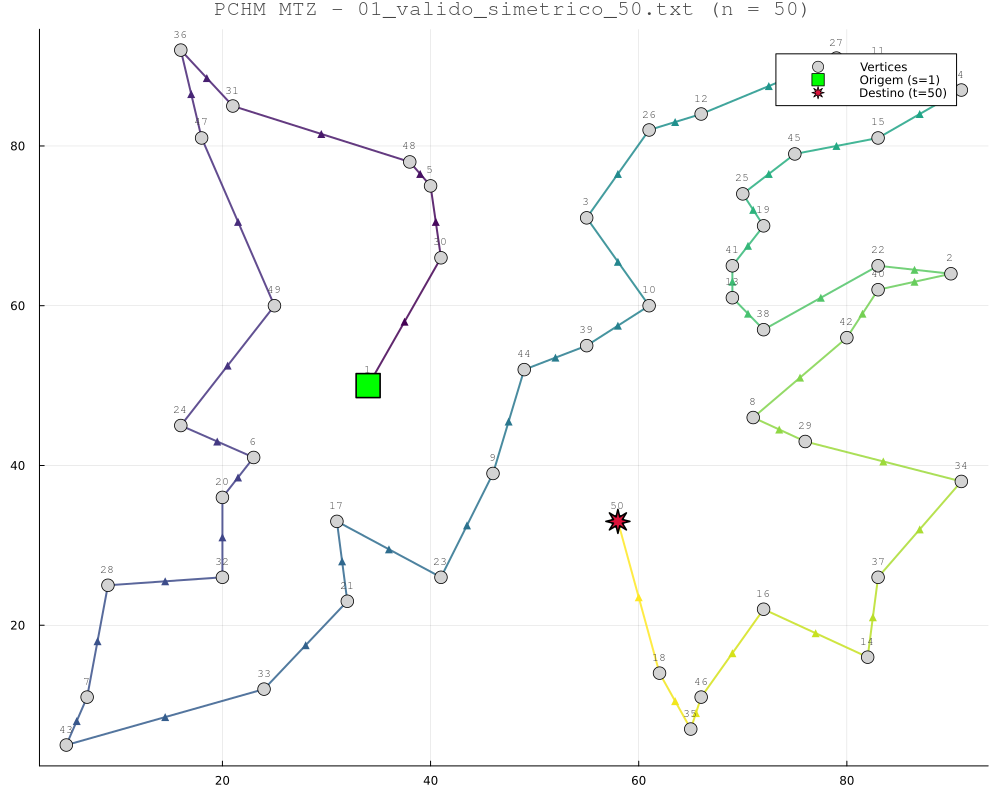
\includegraphics[width=\linewidth]{graficos/01_valido_simetrico_50.png}
\caption{\texttt{01\_valido\_simetrico\_50} ($n=50$, custo 512,90)}
\end{minipage}
\hfill
\begin{minipage}{0.48\textwidth}
\centering
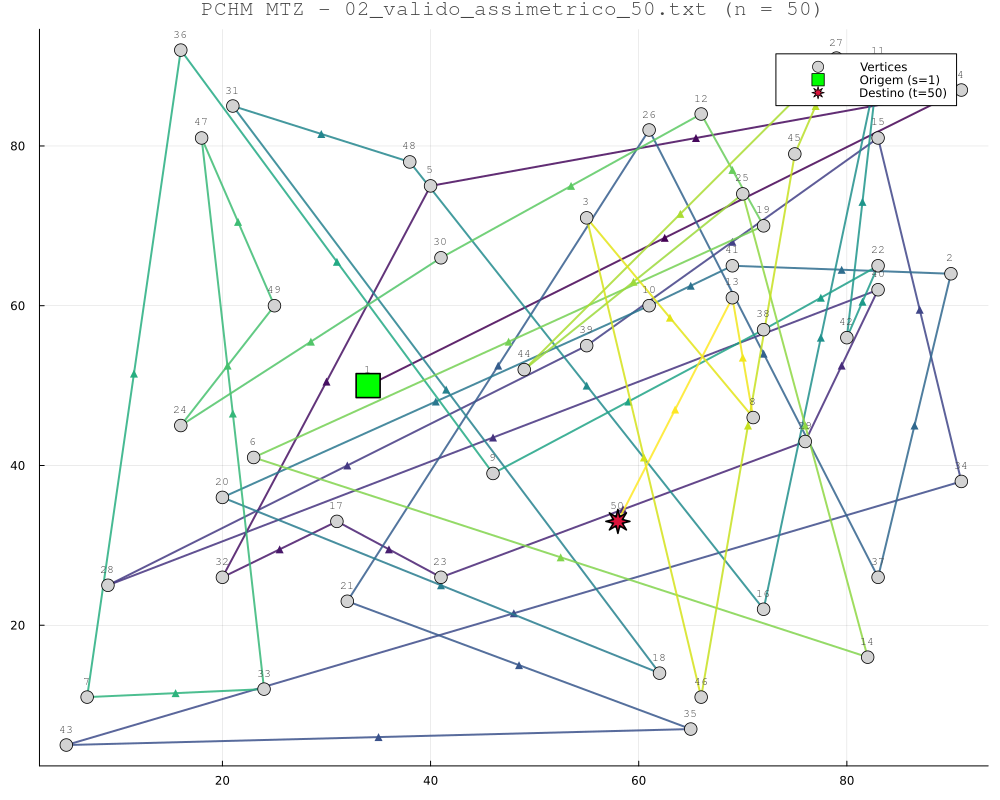
\includegraphics[width=\linewidth]{graficos/02_valido_assimetrico_50.png}
\caption{\texttt{02\_valido\_assimetrico\_50} ($n=50$, custo 574,60)}
\end{minipage}
\end{figure}

\begin{figure}[H]
\centering
\begin{minipage}{0.32\textwidth}
\centering
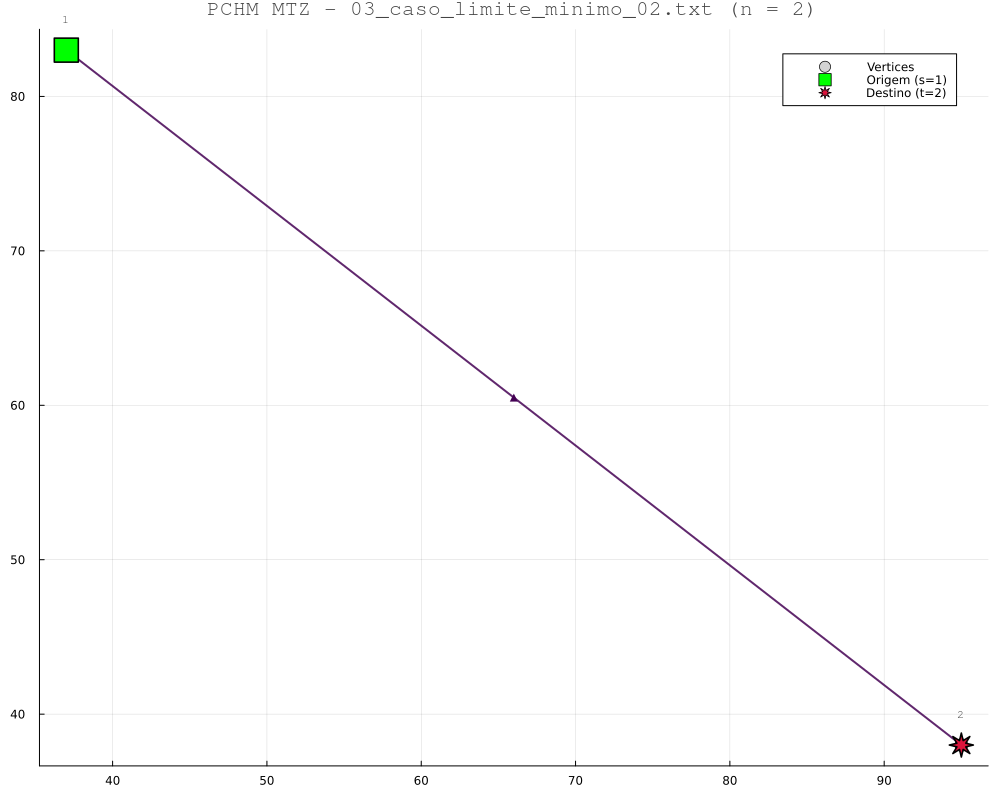
\includegraphics[width=\linewidth]{graficos/03_caso_limite_minimo_02.png}
\caption{\texttt{03\_caso\_limite\_02} ($n=2$, custo 15,00)}
\end{minipage}
\hfill
\begin{minipage}{0.32\textwidth}
\centering
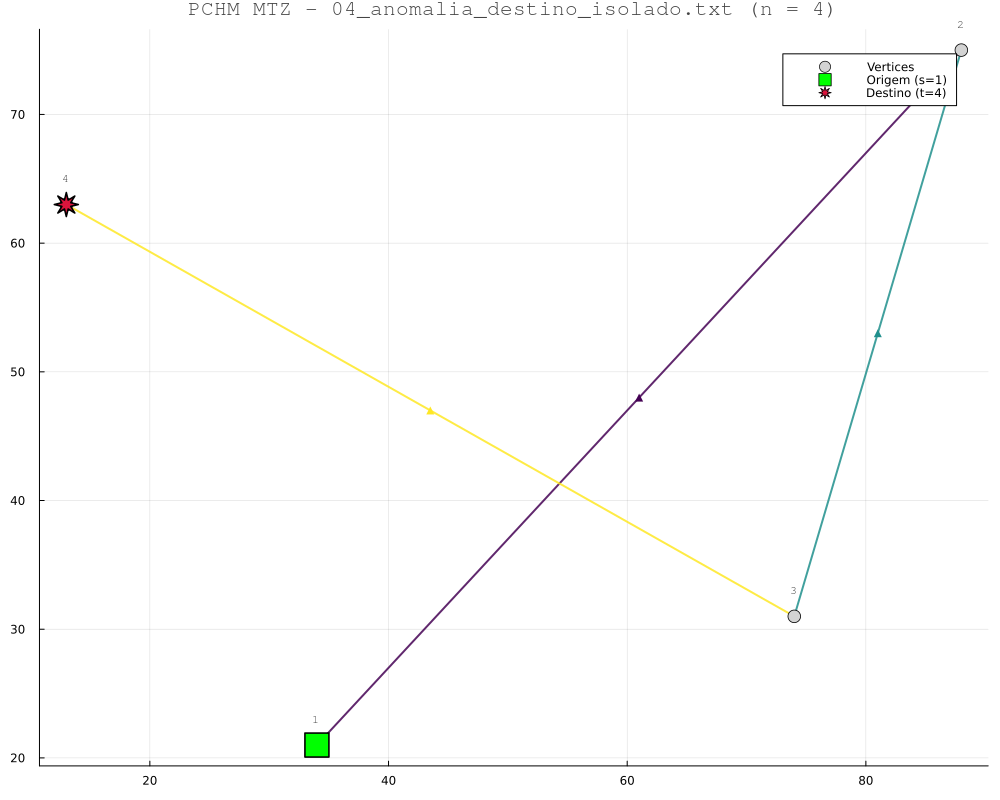
\includegraphics[width=\linewidth]{graficos/04_anomalia_destino_isolado.png}
\caption{\texttt{04\_destino\_isolado} ($n=4$, custo 10024,00)}
\end{minipage}
\hfill
\begin{minipage}{0.32\textwidth}
\centering
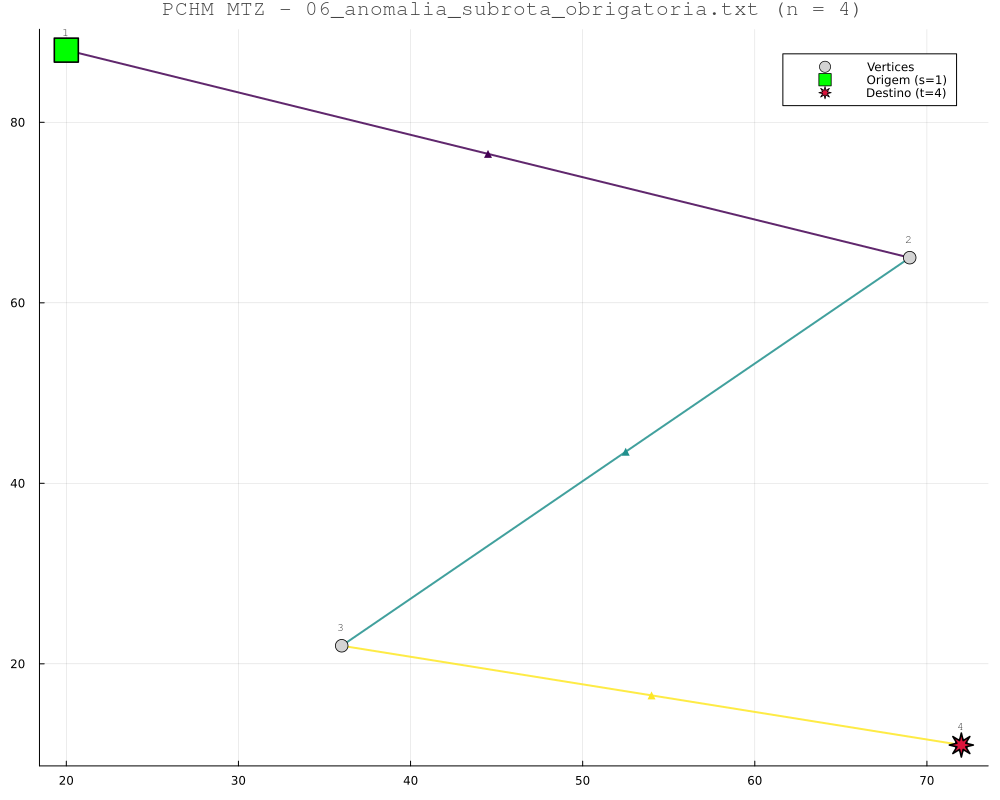
\includegraphics[width=\linewidth]{graficos/06_anomalia_subrota_obrigatoria.png}
\caption{\texttt{06\_subrota\_obrig.} ($n=4$, custo 20008,00)}
\end{minipage}
\end{figure}

\subsection{Instâncias da TSPLIB}

\begin{figure}[H]
\centering
\begin{minipage}{0.48\textwidth}
\centering
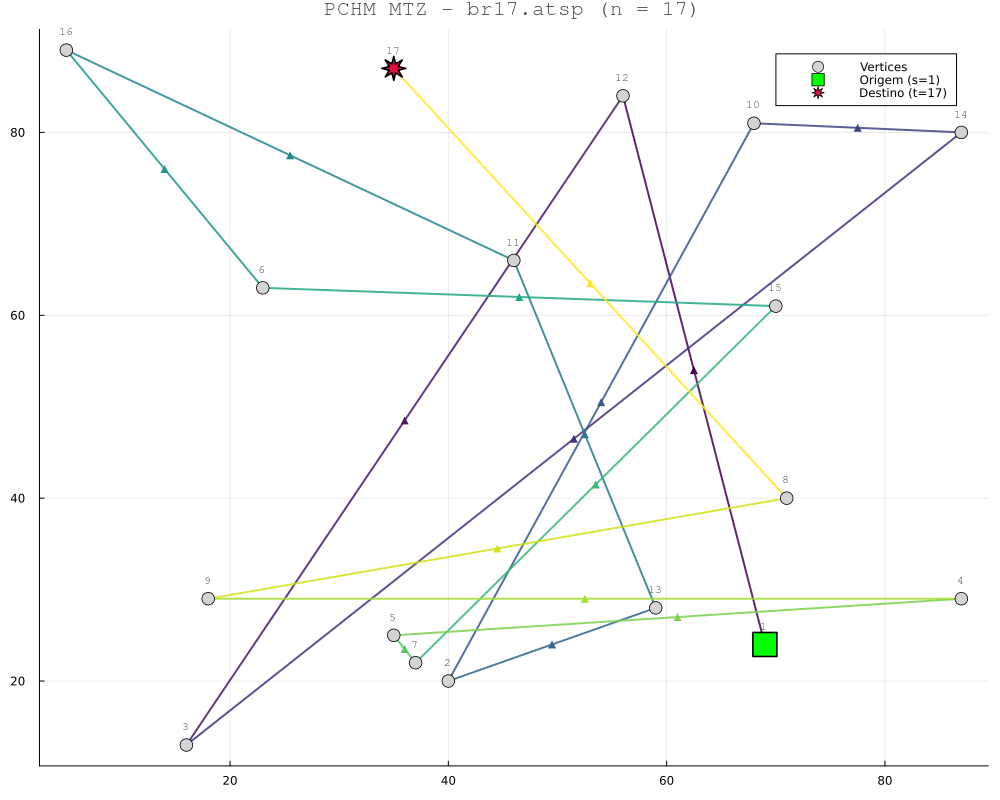
\includegraphics[width=\linewidth]{graficos/br17.png}
\caption{\texttt{br17.atsp} ($n=17$, custo 34,00)}
\end{minipage}
\hfill
\begin{minipage}{0.48\textwidth}
\centering
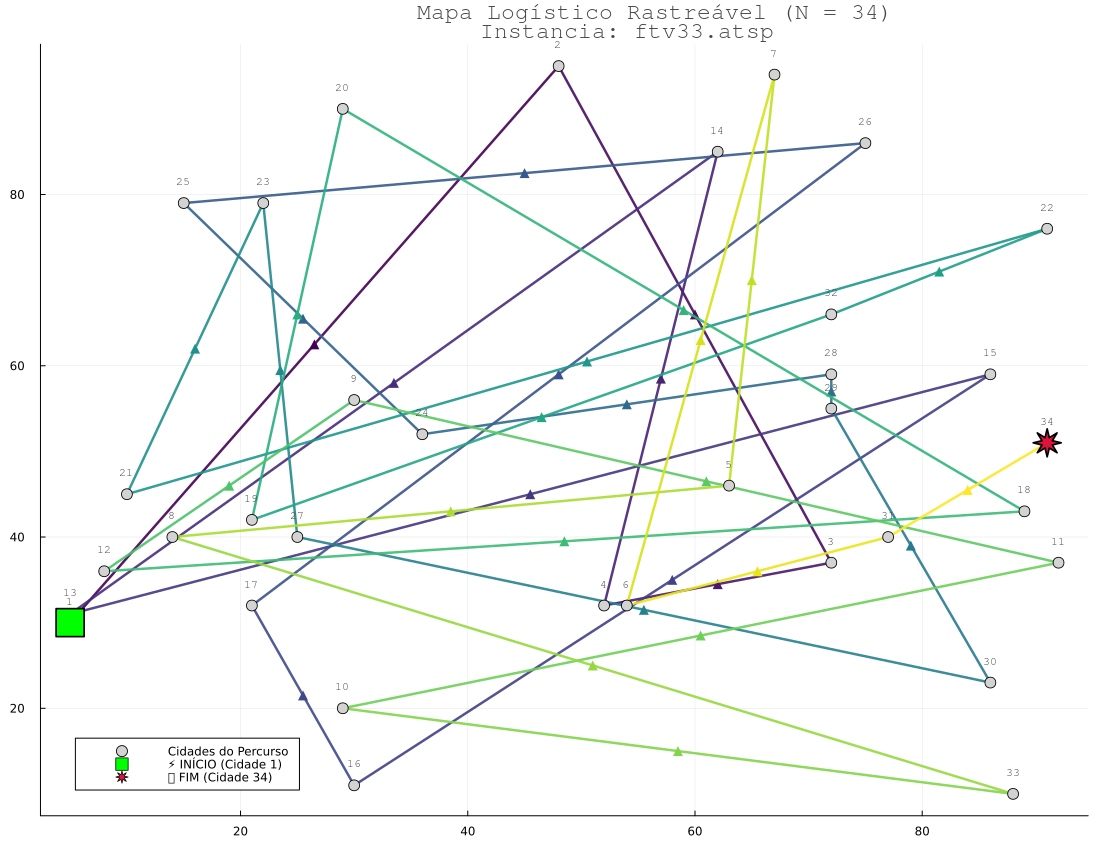
\includegraphics[width=\linewidth]{graficos/ftv33.png}
\caption{\texttt{ftv33.atsp} ($n=34$, custo 1275,00)}
\end{minipage}
\end{figure}

\begin{figure}[H]
\centering
\begin{minipage}{0.48\textwidth}
\centering
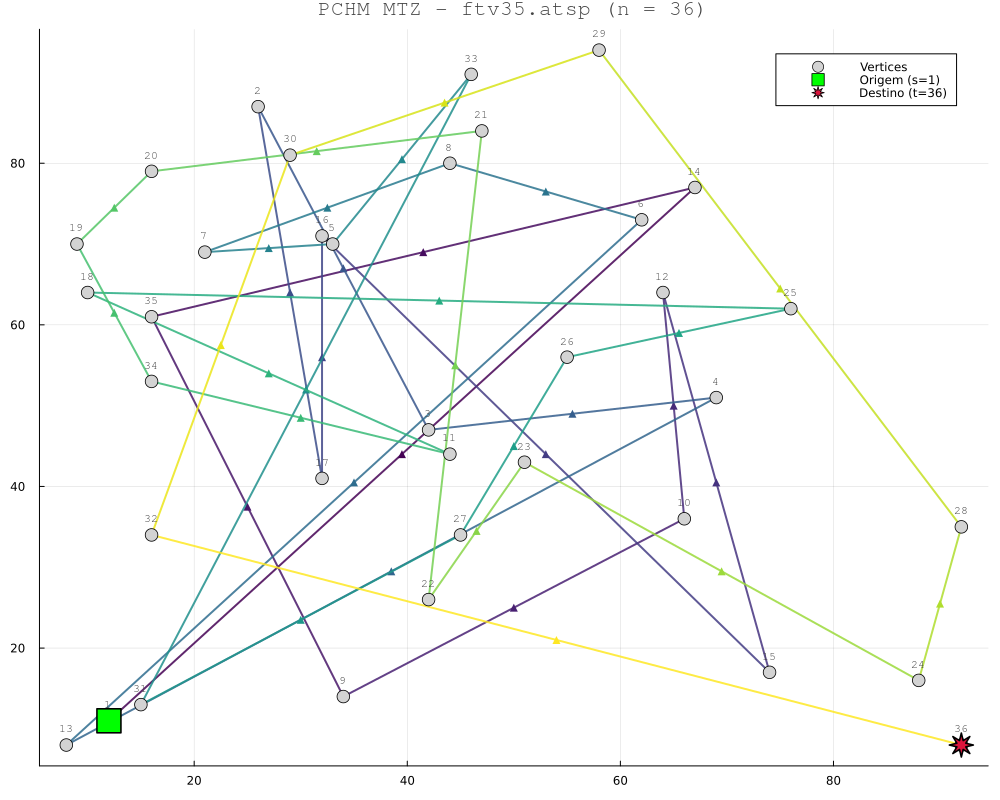
\includegraphics[width=\linewidth]{graficos/ftv35.png}
\caption{\texttt{ftv35.atsp} ($n=36$, custo 1443,00)}
\end{minipage}
\hfill
\begin{minipage}{0.48\textwidth}
\centering
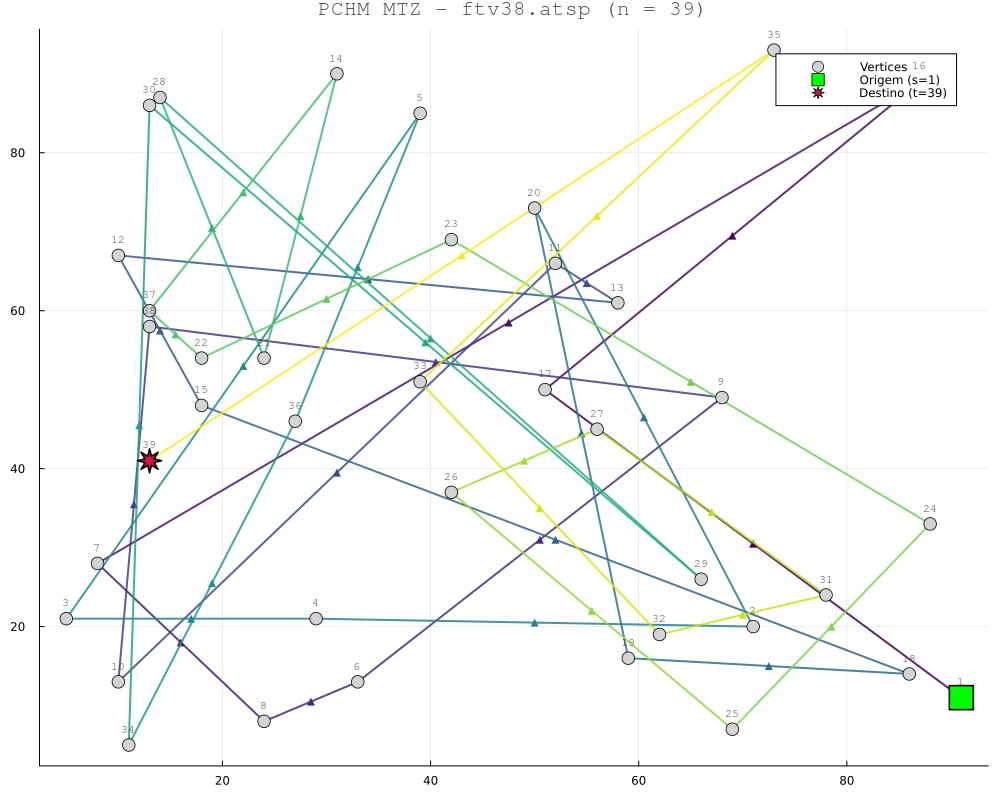
\includegraphics[width=\linewidth]{graficos/ftv38.png}
\caption{\texttt{ftv38.atsp} ($n=39$, custo 1511,00)}
\end{minipage}
\end{figure}

\begin{figure}[H]
\centering
\begin{minipage}{0.48\textwidth}
\centering
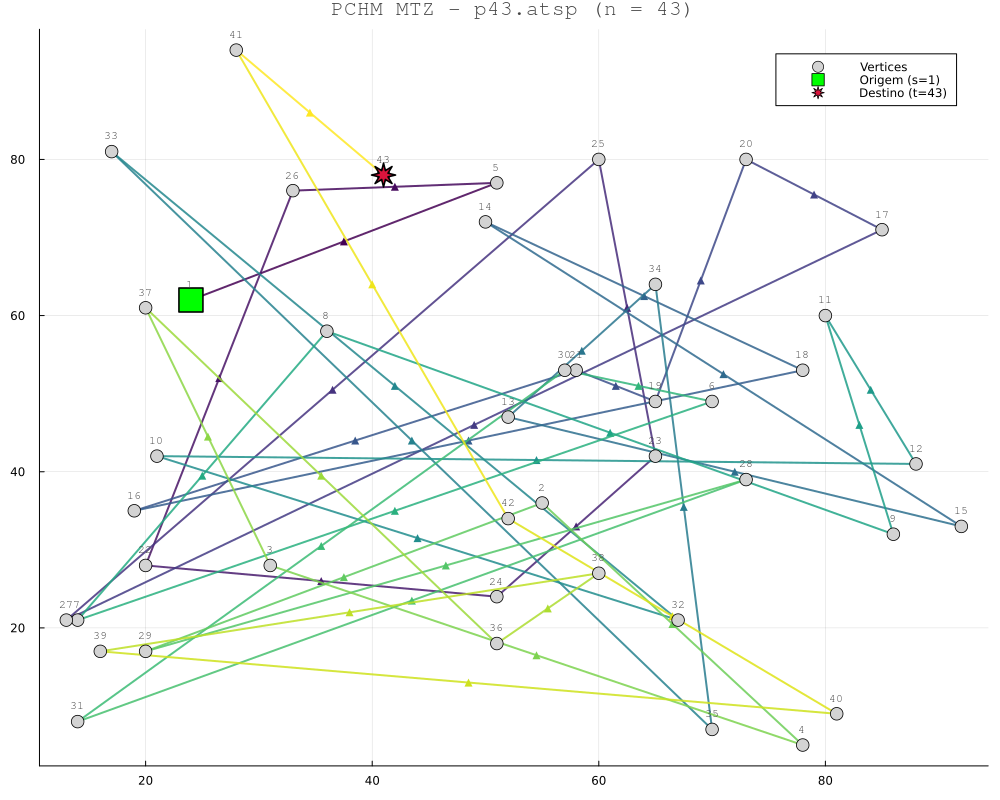
\includegraphics[width=\linewidth]{graficos/p43.png}
\caption{\texttt{p43.atsp} ($n=43$, custo 589,00)}
\end{minipage}
\hfill
\begin{minipage}{0.48\textwidth}
\centering
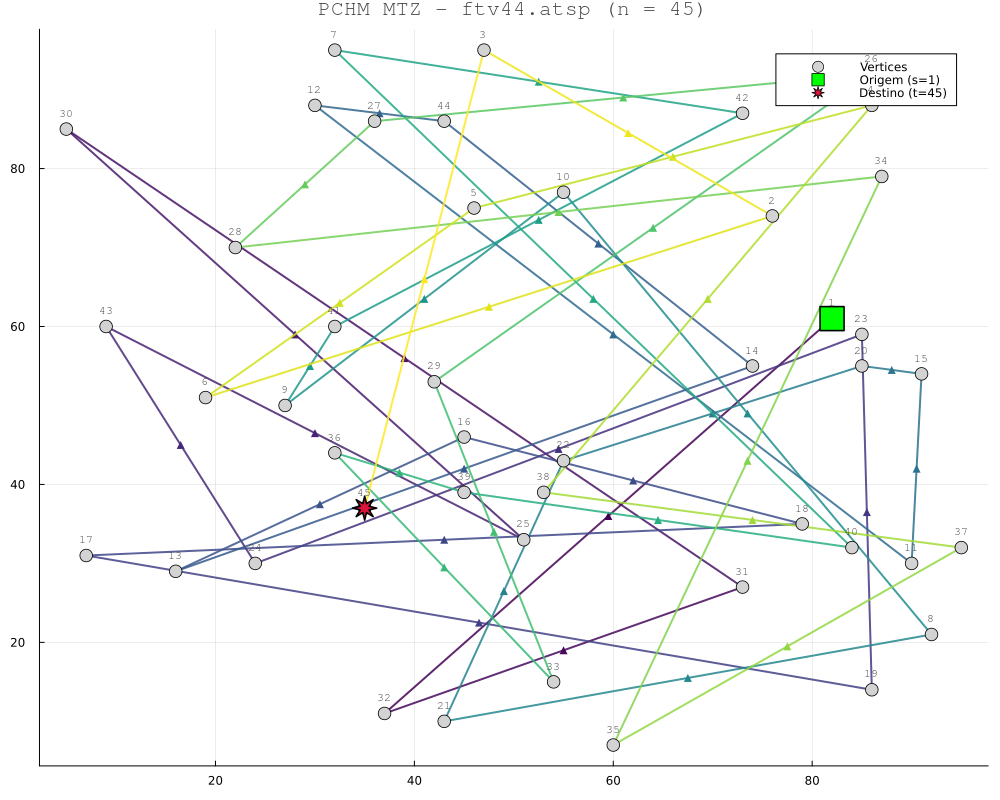
\includegraphics[width=\linewidth]{graficos/ftv44.png}
\caption{\texttt{ftv44.atsp} ($n=45$, custo 1614,00)}
\end{minipage}
\end{figure}

\begin{figure}[H]
\centering
\begin{minipage}{0.48\textwidth}
\centering
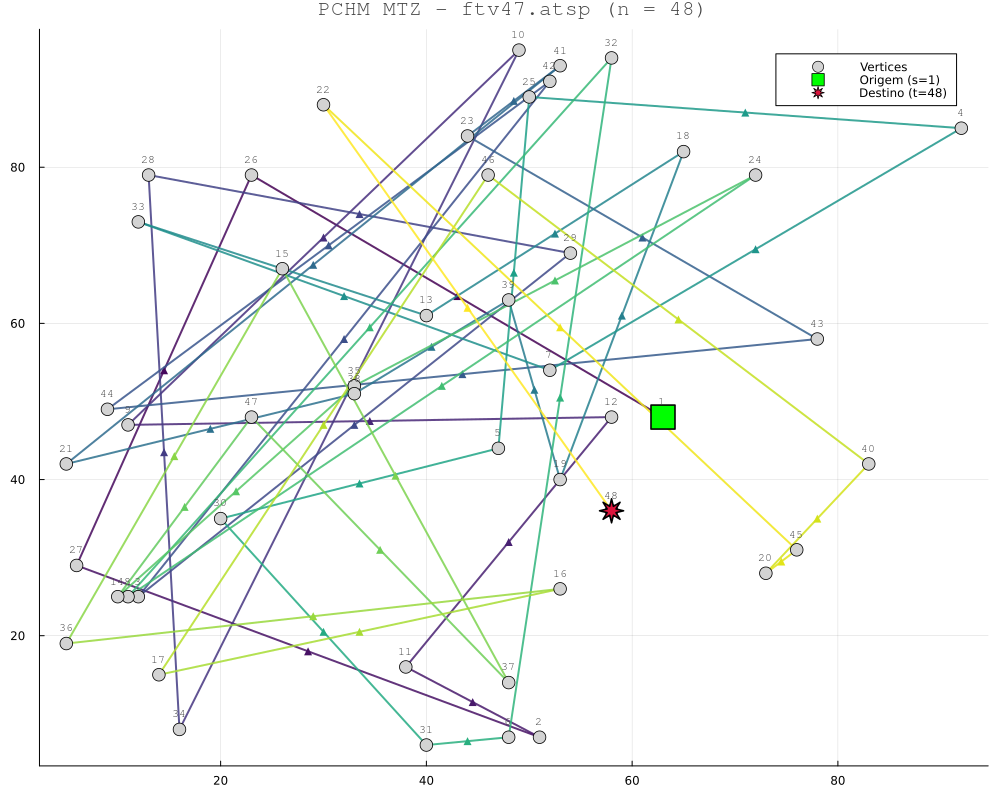
\includegraphics[width=\linewidth]{graficos/ftv47.png}
\caption{\texttt{ftv47.atsp} ($n=48$, custo 1754,00)}
\end{minipage}
\hfill
\begin{minipage}{0.48\textwidth}
\centering
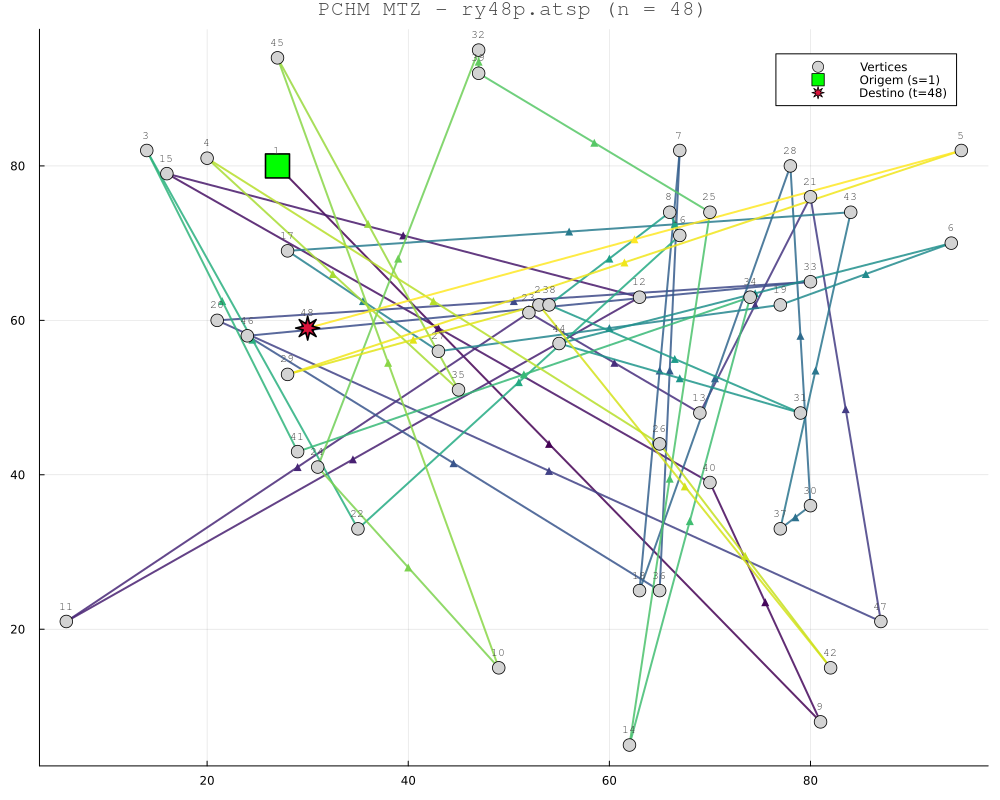
\includegraphics[width=\linewidth]{graficos/ry48p.png}
\caption{\texttt{ry48p.atsp} ($n=48$, custo 14070,00)}
\end{minipage}
\end{figure}

\begin{figure}[H]
\centering
\begin{minipage}{0.48\textwidth}
\centering
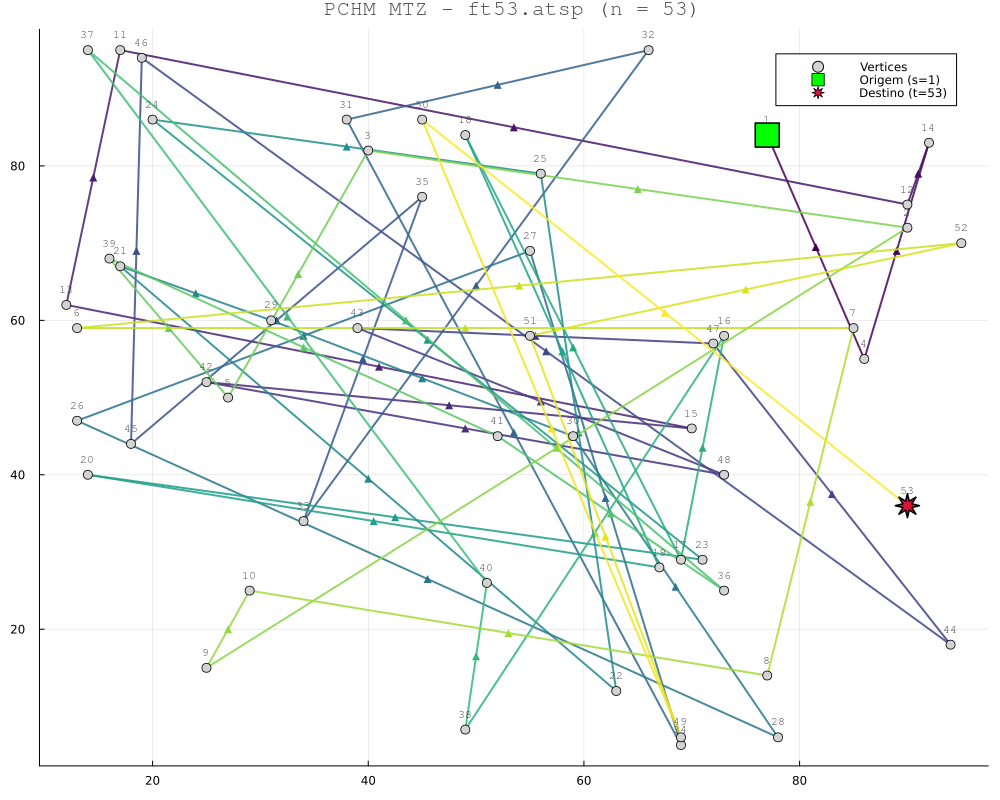
\includegraphics[width=\linewidth]{graficos/ft53.png}
\caption{\texttt{ft53.atsp} ($n=53$, custo 6196,00)}
\end{minipage}
\hfill
\begin{minipage}{0.48\textwidth}
\centering
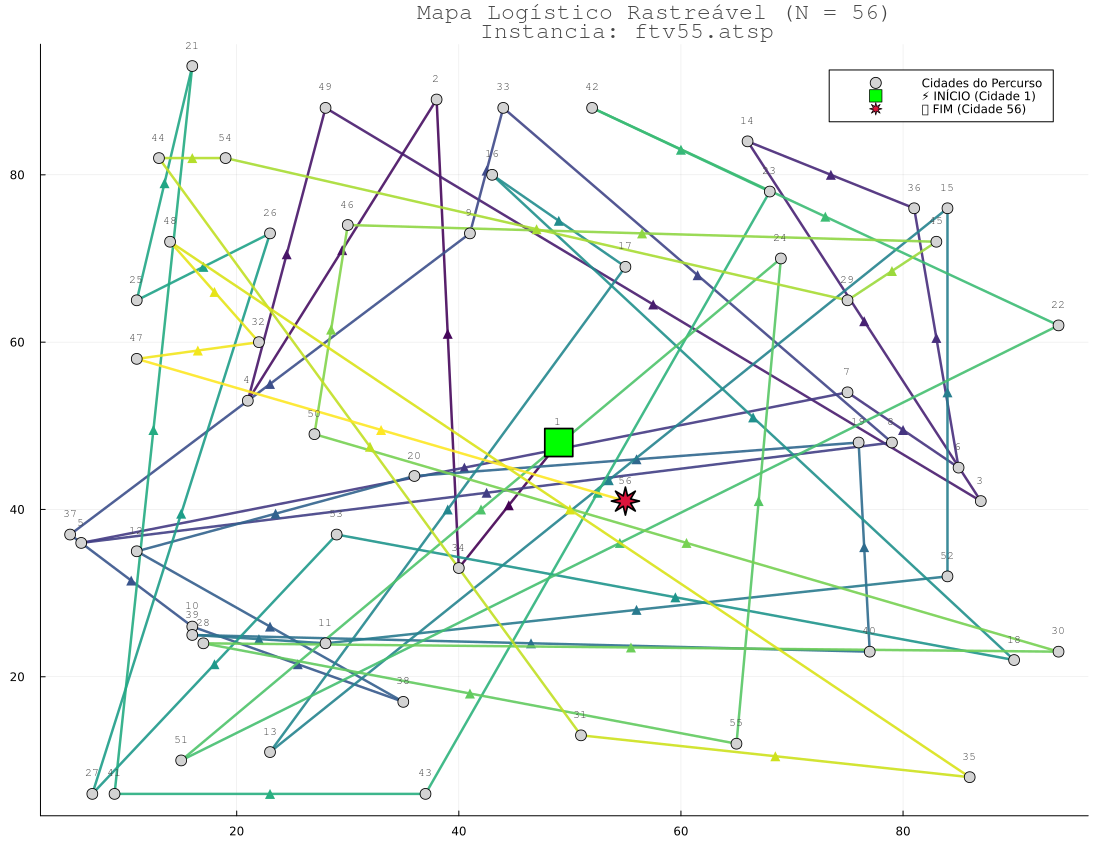
\includegraphics[width=\linewidth]{graficos/ftv55.png}
\caption{\texttt{ftv55.atsp} ($n=56$, custo 1613,00)}
\end{minipage}
\end{figure}

\begin{figure}[H]
\centering
\begin{minipage}{0.48\textwidth}
\centering
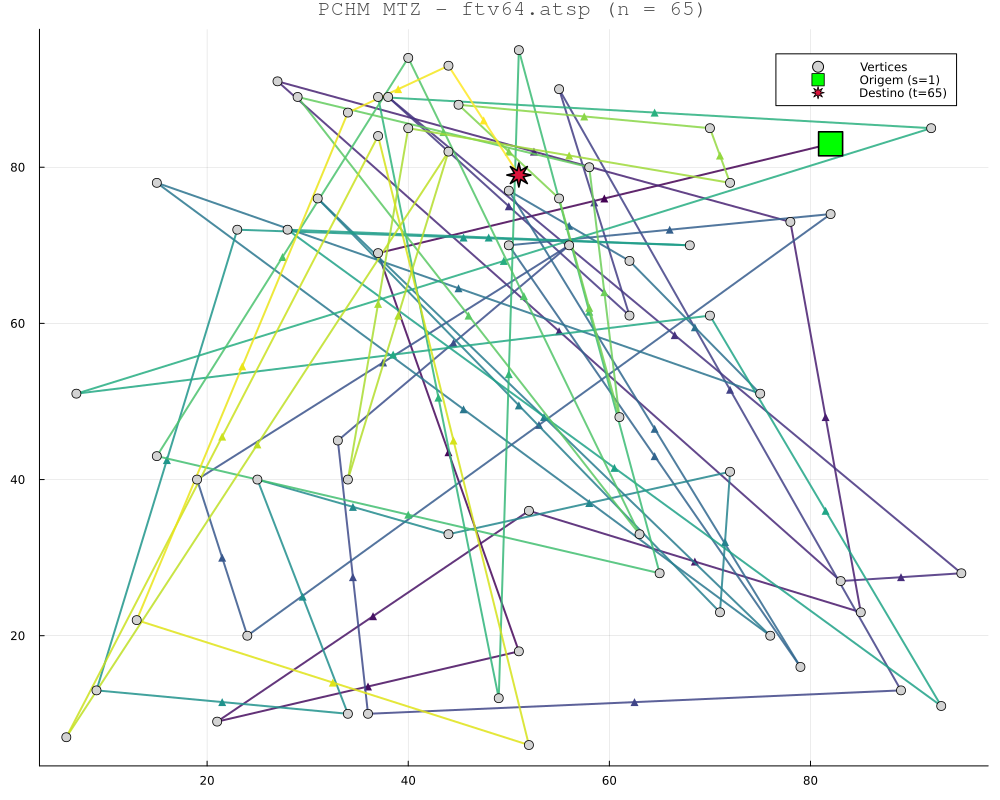
\includegraphics[width=\linewidth]{graficos/ftv64.png}
\caption{\texttt{ftv64.atsp} ($n=65$, custo 1840,00)}
\end{minipage}
\hfill
\begin{minipage}{0.48\textwidth}
\centering
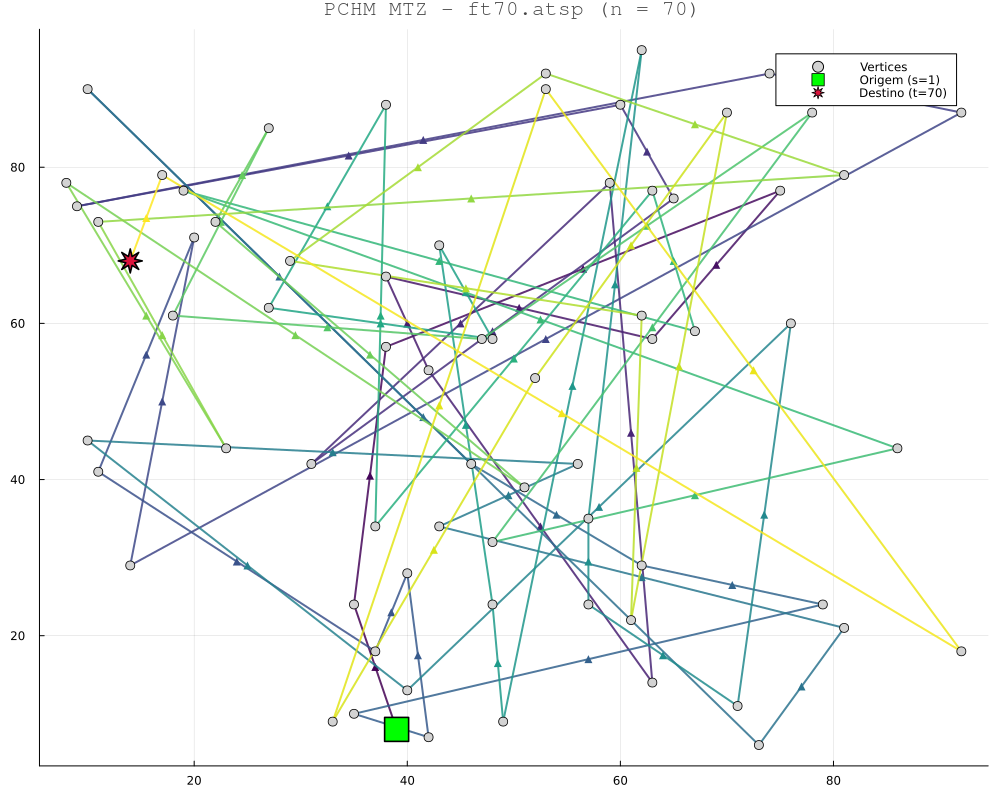
\includegraphics[width=\linewidth]{graficos/ft70.png}
\caption{\texttt{ft70.atsp} ($n=70$, custo 37655,00)}
\end{minipage}
\end{figure}

\begin{figure}[H]
\centering
\begin{minipage}{0.48\textwidth}
\centering
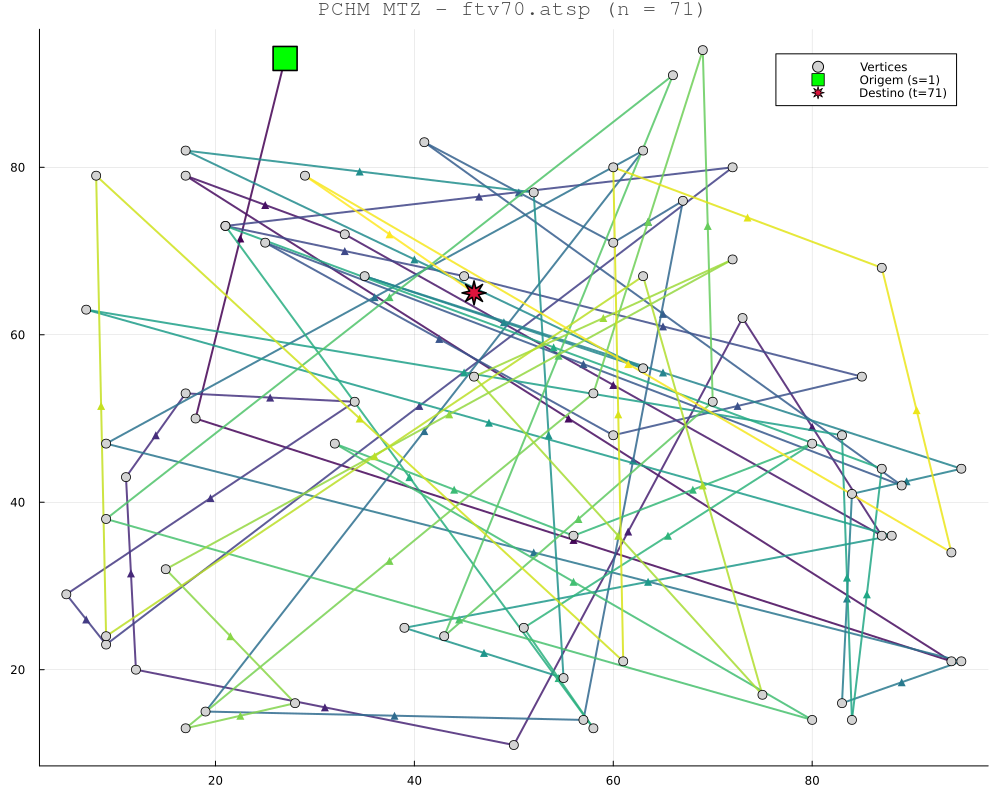
\includegraphics[width=\linewidth]{graficos/ftv70.png}
\caption{\texttt{ftv70.atsp} ($n=71$, custo 1958,00)}
\end{minipage}
\end{figure}

\section{Declaração de Uso de Inteligência Artificial (Atividade 4)}
Foi usada como apoio na construção do código busca de artigos sobre a formulação e redação do relátorio.
\end{document}
